\documentclass[11pt, a4paper]{article}

\usepackage{color}

\usepackage{amsmath}
\usepackage{amssymb}
\usepackage[pdftex]{graphicx}
\usepackage{alltt}
\usepackage{caption}
\usepackage{subcaption}
\usepackage{epstopdf}


\author{Yacine Derouach, Stefan Hegglin, Huub Heijnen, Elise Ledieu}
\title{Epidemic models of Flu outbreaks}
\begin{document}
\maketitle

\section{Model and Data Description}
\subsection{The SIR model}
\label{sec:SIR}
\paragraph{}
The Susceptible-Infected-Recovered (SIR) model is a deterministic model that describes the influenza transmission. We consider the version proposed by Coehlo et al. \cite{coelho2011bayesian}.

\begin{equation}
\frac{dS}{dt} = - \lambda S
\end{equation}
\begin{equation}
\frac{dI}{dt} = \lambda S - \tau R
\end{equation}
\begin{equation}
\frac{dR}{dt} = \tau R
\end{equation}

with \[ \lambda = \beta (\alpha I + m) \]

where $S$ is the normalized number of susceptible individuals, $I$is the normalized number of infected individuals, $R$ is the normalized number of recovered individuals, $\tau $ is the recovery rate, $\beta $ is the transmission rate, $\alpha$ is the ratio of symptomatic infection and m is the infectious migration rate.

\begin{figure}[h]
\center
   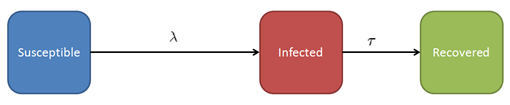
\includegraphics[width = \textwidth]{picture1.png}
   \caption{Compartmental representation of the SIR model}
   \label{SIRcr}
\end{figure}

$\beta$ is time-dependent and models the seasonality of the flu epidemics. Here,every season is considered as independent of the other ones. The parameters are optimized on a data set only containing winter months, where the epidemy occurs. $\beta$ is here set to 50, as a scaling parameter for the other parameters $\alpha$ and $\tau$.

The set of parameters to be determined in this case is : $ {\alpha, \tau, m, S_o}$. $S_o$ is the number of susceptible individuals at the beginning at each season. The parameters $m$ and $\tau$ do not depend on the season considered, whereas the parameters $\alpha$ and $S_o$ change at each season.

\subsection{The SEIR model}
\paragraph{}
The Susceptible-Exposed-Infected-Recovered (SEIR) model is an extension of the SIR model. We added the Exposed category to the previous system.

\begin{equation}
\frac{dS}{dt} = - \lambda S
\end{equation}
\begin{equation}
\frac{dE}{dt} = \lambda S - \gamma E
\end{equation}
\begin{equation}
\frac{dI}{dt} = \gamma E - \tau R
\end{equation}
\begin{equation}
\frac{dR}{dt} = \tau R
\end{equation}

with \[ \lambda = \beta (\alpha I + m) \]

where $E$ is the normalized number of exposed individuals and $\gamma$ is the transition rate from latent to infected state.

\begin{figure}[h]
\center
   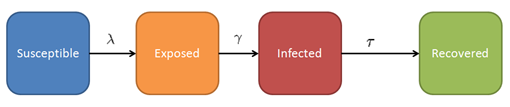
\includegraphics[width = \textwidth]{picture2.png}
   \caption{Compartmental representation of the SEIR model}
   \label{SEIRcr}
\end{figure}

$\beta$ has the same behavior in this model and in the SIR model (Section \ref{sec:SIR}).

The set of parameters to be determined in this model is : $ { \alpha, \gamma, \tau, m, S_o}$. Here, we suppose that $\gamma$ is constant for all the seasons. 

\subsection{Data}
\paragraph{}
The data set used is the one provided by Google Flu Trends. The data is made of the number of infected people reported weekly between December 2011 and May 2014. This time span correspond to three flu seasons. A flu season is considered to begin in December, as the peak of the flu is observed in February in the European countries \cite{baumgartner2012seasonality}. The data was normalized. 

\section{Likelihood}
\paragraph{}
The likelihood of the parameters is 
\begin{equation}
L(\Theta) = L(\Phi) = \prod_{t=1}^T p( d(t) | \Phi(t),I) 
\label{eq:likelihood}
\end{equation}

assuming normal errors with fixed variance $\sigma^2$
\begin{equation}
p(d(t) | \Phi(t),I) = \frac{1}{\sqrt{2\pi}\sigma} \exp^{-\frac{1}{2\sigma^2}[y(t) - I(x(t), \Theta)]}
\label{eq:gaussianPrior}
\end{equation}

where $I(x(t), \Theta)$ is the number of infected people at time $t$ predicted by the model given the input values $x(t)$ ; $y(t)$ is the observed data ; $d(t)$ is the data at a time point.

$I(x(t), \Theta)$ corresponds to the solution of an ODE system. There may be no simple analytical solution for this one and therefore, no analytical derivation possible of it. It depends indeed on the parameter $\beta$, which is time-dependent.

\section{Priors}
\paragraph{}
Thanks to the article by Coehlo et al. \cite{coelho2011bayesian}, it is possible to use informative priors for the SIR model. By analogy, the information on the parameters in the SIR model is reused to determine the priors of the SEIR model. The $\gamma$ parameter has an uninformative prior (a uniform distribution between 0 and 1). Moreover, the prior over $\tau$ is considered to be uniform between 1 and 2, as it was derived experimentally in the article of Coehlo et al.\cite{coelho2011bayesian}. 

Here are the priors used for each parameter : 
\begin{itemize}
\item $\alpha \sim \mathcal{U}(0, 0.4)$ 
\item $\gamma \sim \mathcal{U}(0, 1)$
\item $\tau \sim \mathcal{U}(1, 2)$
\item $m \sim  \mathcal{U}(0, 4e-6)$
\item $S_o \sim \mathcal{U}(0, 1)$
\end{itemize}

\section{Optimisation and Uncertainty of the parameters}

\subsection{Method : Delayed Rejection Markov Chain Monte Carlo}

To find a good parameter fit, two steps were used : firstly, $\tau$ was fixed to the value $1.4$ as proposed by \cite{coelho2011bayesian} and the other parameters were fitted using the DRAM algorithm. Secondly, the constraint over $\tau$ was released and $\tau$ was optimized given the optimal values of the parameters found in the first step

In Belgium, the parameters found by the DRAM algorithm are given in table \ref{tab:sirDRAM} for the SIR model and in table \ref{tab:seirDRAM} for the SEIR model.

\begin{table}[h]
\centering
\begin{tabular}{| c | c | c |}
    \hline
    Parameter & Season & Optimal Value &  Standard Deviation\\ \hline
    \multirow{1}{*}{$\alpha$} & 2010 & 0.1525 & 0 \\ \hline
    \multirow{1}{*}{$\tau$} & 2010 & 1.7357 & 0 \\ \hline
    \multirow{1}{*}{$m$} & 2010 & 2.7e-6 & 0 \\ \hline
    \multirow{1}{*}{$S_o$} & 2010 & 0.2743 & 0 \\
    \hline  
    \end{tabular}
    \caption{Optimal parameters found for the SIR model in Belgium}
    \label{tab:sirDRAM}
\end{table}

\begin{table}[h]
\centering
\begin{tabular}{| c | c | c |}
    \hline
    Parameter & Season & Optimal Value &  Standard Deviation\\ \hline
    \multirow{1}{*}{$\alpha$} & 2010 & 0.1525 & 0 \\ \hline
    \multirow{1}{*}{$\gamma$} & 2010 & 0 & 0 \\ \hline
    \multirow{1}{*}{$\tau$} & 2010 & 1.7357 & 0 \\ \hline
    \multirow{1}{*}{$m$} & 2010 & 2.7e-6 & 0 \\ \hline
    \multirow{1}{*}{$S_o$} & 2010 & 0.2743 & 0 \\
    \hline  
    \end{tabular}
    \caption{Optimal parameters found for the SEIR model in Belgium}
    \label{tab:seirDRAM}
\end{table}
  

\subsection{Method : Asymptotic Approximation}
\paragraph{}
Analytically, the Log Posterior function is 

\begin{equation}
l(\Theta) \propto - log(L(\Theta)) - log(\pi(\Theta))
\end{equation}

where $\pi(\Theta)$ is the prior distribution of the parameters.

As gaussian errors are assumed (Equation \ref{eq:gaussianPrior}),

\begin{equation}
l(\Theta) \propto \frac{T}{2} log(\sigma^2) + \frac{1}{2 \sigma^2} \sum_{t=1}^T (y(t)-I(x(t), \Theta))^2 - log(\pi(\Theta))
\end{equation}

The best estimate can thus be derived by $\frac{\partial l}{\partial \Theta}(\Theta^*) = 0$. The following formula is then obtained :

\begin{equation}
\sum_{t=1}^T (y(t) - I(x(t), \Theta^*)) \frac{\partial I(x(t), \Theta^*)}{\partial \Theta} = 0
\end{equation}

The optimal model parameters can be retrieved by solving a least square optimization problem. 

The spread of uncertainty is modelled by the Hessian :

\begin{equation}
H(\Theta^*) = \frac{\partial^2 l}{\partial \Theta^2} (\Theta^*) 
\end{equation}

As there is no analytical formulation of the solution $I(x(t), \Theta)$, we use Matlab to solve this.


\bibliographystyle{plain}
\bibliography{references.bib}

\end{document}
